\section{自动合成配件}

\subsection{配置}

打开 \lstinline{Setting.lua} 文件,配置如下坐标。

\textbf{\color{red}注意:配置文件修改后后,需要在罗技软件中重新导入并运行以使配置生效。}

\begin{figure}[H]
    \Centering
    \parbox[l]{\textwidth}{\lstinline{CRAFT_PARTS_AUTO_FILL_X}、\lstinline{CRAFT_PARTS_AUTO_FILL_Y}:“自动添加”按钮坐标位置(图 \ref{ch3fig-auto-fill})。}
    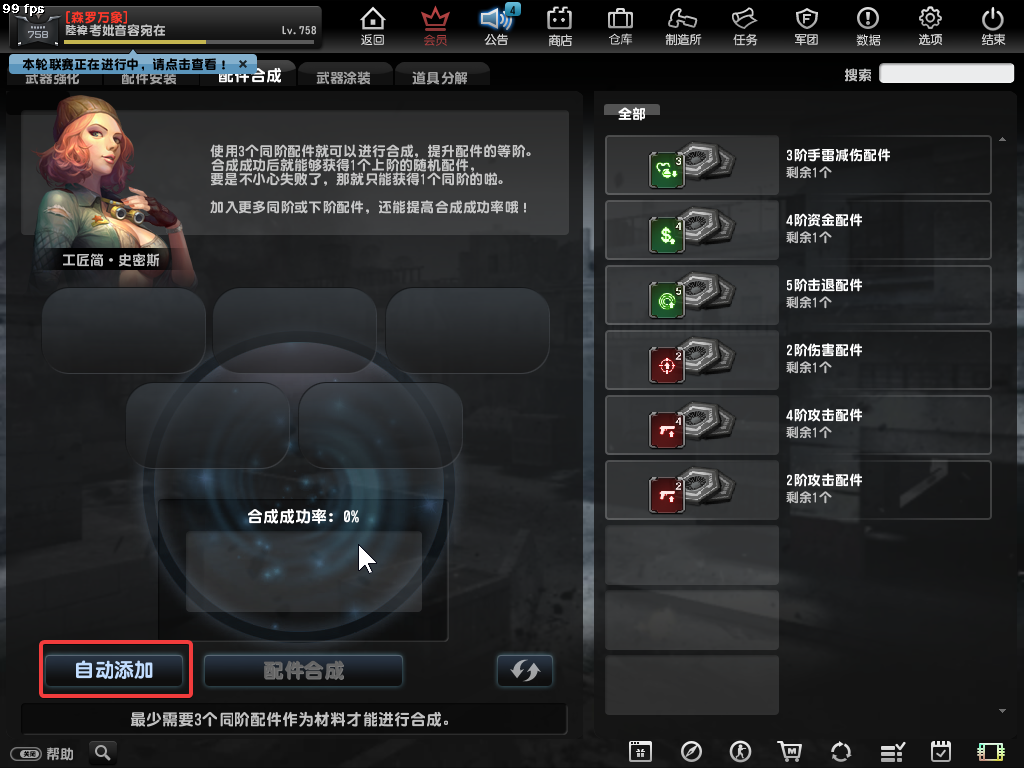
\includegraphics[width=\textwidth]{docs/assets/auto_fill.png}
    \caption{“自动添加”按钮}
    \label{ch3fig-auto-fill}
\end{figure}
\clearpage

\begin{figure}[H]
    \Centering
    \parbox[l]{\textwidth}{\lstinline{CRAFT_PARTS_COMBINE_X}、\lstinline{CRAFT_PARTS_COMBINE_Y}:“合成配件”按钮坐标位置(图 \ref{ch3fig-combine})。}
    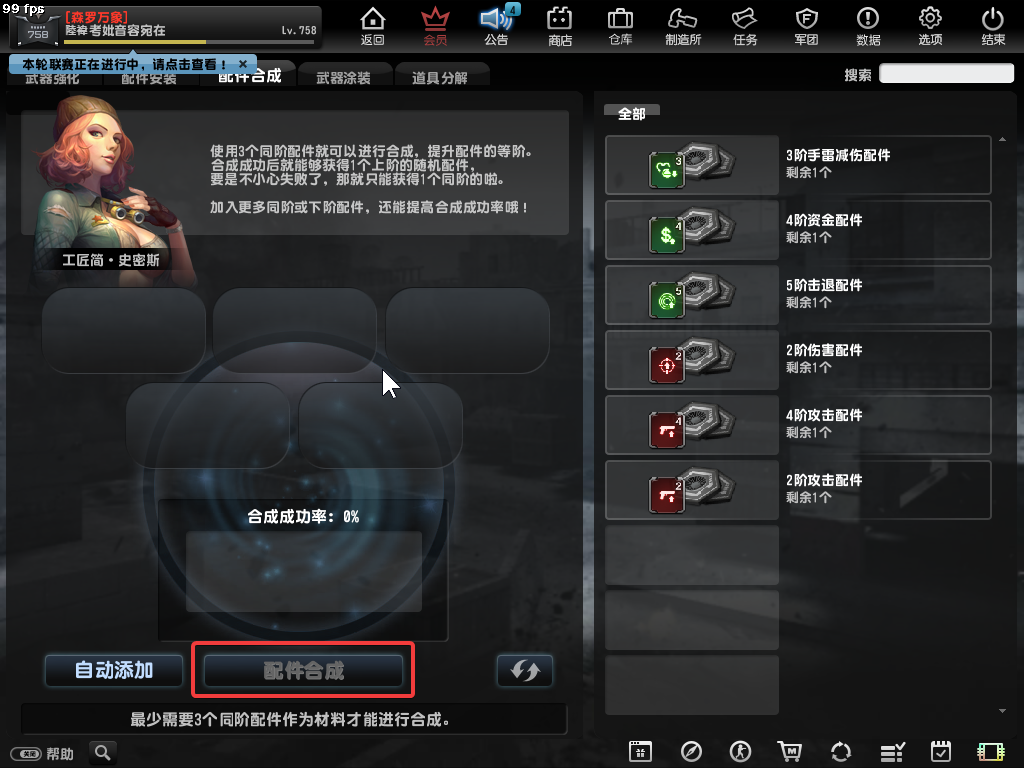
\includegraphics[width=\textwidth]{docs/assets/combine.png}
    \caption{“合成配件”按钮}
    \label{ch3fig-combine}
\end{figure}
\clearpage

\begin{figure}[H]
    \Centering
    \parbox[l]{\textwidth}{\lstinline{CRAFT_PARTS_CLEAR_X}、\lstinline{CRAFT_PARTS_CLEAR_Y}:“清空”按钮坐标位置(图 \ref{ch3fig-clear})。}
    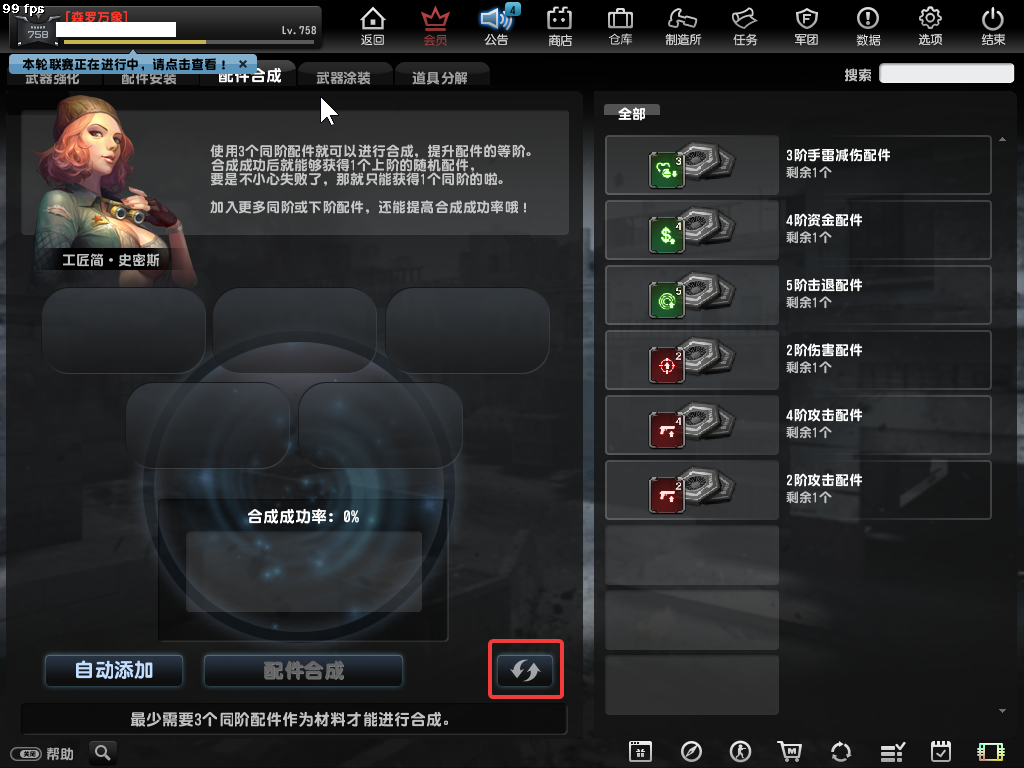
\includegraphics[width=\textwidth]{docs/assets/clear.png}
    \caption{“清空”按钮}
    \label{ch3fig-clear}
\end{figure}
\clearpage

\subsection{使用方法}

在 0 模式下,提前合成一次配件输入仓库密码。
随后,切换到 3 模式,配件将自动开始合成。
切换回 0 模式,配件合成将停止。